\documentclass[a4 paper]{article}
\usepackage{amssymb, amsmath, graphicx, float, color, geometry}
\geometry{top=30mm}

%opening
\title{Drugs And Their Impact On American Society}
\author{Colin Van Oort\\DVO Group Inc.}
\date{\vspace{-5ex}}

\begin{document}

\maketitle


\begin{abstract}
\noindent Drugs are a massive problem in the United States. Each year the federal government spends roughly \$1.4 billion on anti-drug ad campaigns and public service announcements, as well as about \$11 billion on drug treatment programs such as Narcotics Overdose Prevention and Education, Not My Kid, and Robert Crown Center Heroin Prevention Program \cite{Anti-Drug Money}. With that much money being thrown around it makes sense to identify the drugs which cause the most damage to society and patterns related to usage of those drugs. Such information could be used to ensure that resources are being allocated appropriately and society can get the largest benefit for their money. In an attempt to provide such information an investigation of U.S. drug usage was performed via data analysis of several large, nationally representative data sets. Also, a rough index of the impact that a drug has on society was compiled based off of the number of drug users and the proportion of public services those drug users utilized.
\end{abstract}


\section*{Data \& Methods}

Data from the National Survey on Drug Use and Health (NSDUH, 2002-2013), Drug Abuse Warning Network (DAWN, 2004-2011), and Treatment Episode Data Set - Admissions (TEDS-A, 1992-2012) were obtained in \texttt{.tsv} format and processed using the Python programming language and the csv library. The \texttt{.tsv} format is convenient to access through the csv library and there were little to no inconsistencies in the data sets, thus very little data sanitation was required. After analysis, plots were created using the graphical library matplotlib.


\section*{Results}
The basic process that will be used to calculate the societal impact index (SII) for a certain drug will be the number of users of that drug in a population, multiplied by the proportion of those users who utilize emergency services, multiplied by the proportion of those users who utilize substance abuse treatment services.\\

\noindent The first step towards creating such a SII is the collection and inspection of the required data, drug user populations, drug user emergency service usage, and drug user substance abuse treatment service usage. Along the way we also inspect a couple of other trends in U.S. drug usage data.

\subsection*{What Drugs Are Most Commonly Used?}
The population of users of various drugs is perhaps the simplest statistic to observe, and thus it is the first presented here.

\noindent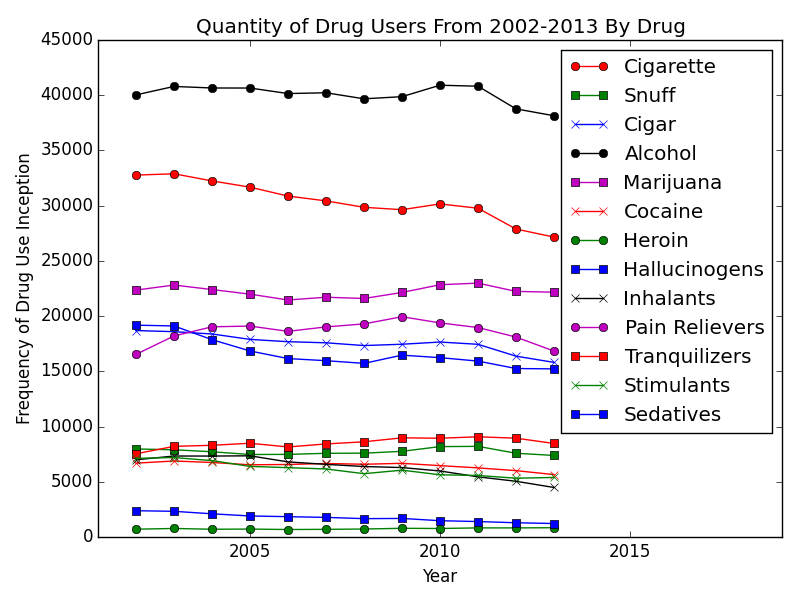
\includegraphics[width=\textwidth]{QDU_02-13}

\noindent Though it is a very simple measure, the relationship between differing drug user populations can provide information on the popularity of a drug and the rough amount of a drug that a society uses.From the plot above it can be seen that the three largest populations are alcohol users, cigarette users, and marijuana users. Another interesting feature is the relative stagnation of most of the populations, it appears that besides the downward trend in alcohol and cigarette users almost all of the other populations are fairly stable. \\

Another useful statistic when comparing drug populations is the average frequency of usage in a drug user population, which may represent a drugs availability or possibly its addictiveness. The average number of days used in a month is a convenient measure of usage frequency because it is a large enough time frame to assess extended usage.

\noindent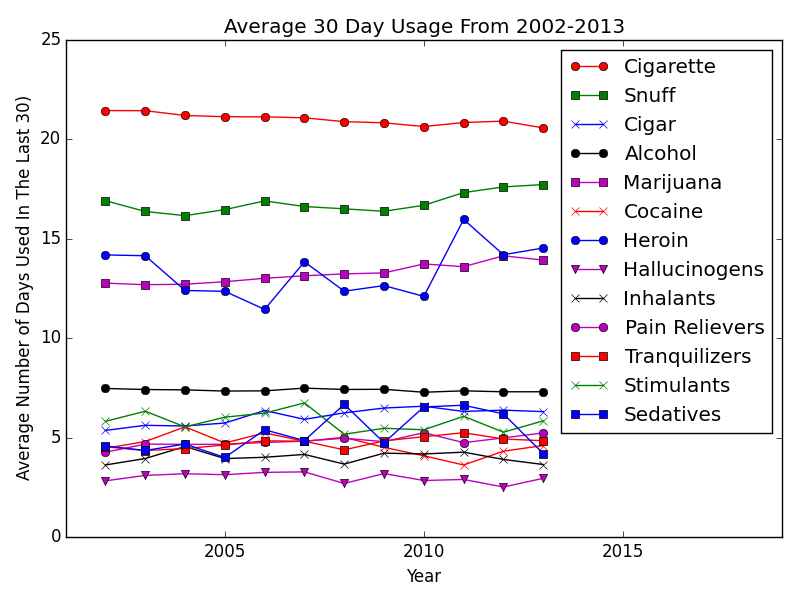
\includegraphics[width=\textwidth]{avgUse30_02-13}

\noindent Similarly to the drug population graph, average drug use frequency appears to be relatively stagnant for most drugs. Notably, cigarette and alcohol usage are in a slight decline, snuff and marijuana usage are increasing, also heroin and sedative usage have experienced relatively wild fluctuations. Cigarettes and snuff have the largest usage, as one may expect of nicotine products due to their availability and addictiveness. While heroin and marijuana are roughly equivalent, with heroin fluctuating above and below marijuana's gradual ascent. 

\subsection*{When Does Drug Use Start?}
Though knowing what drugs to target is highly important with respect to determining how to structure drug education and awareness programs, it's only half of the battle. Knowing what age groups to target with drug education and what time of the year to play drug awareness public announcements are also key pieces of information.\\

\noindent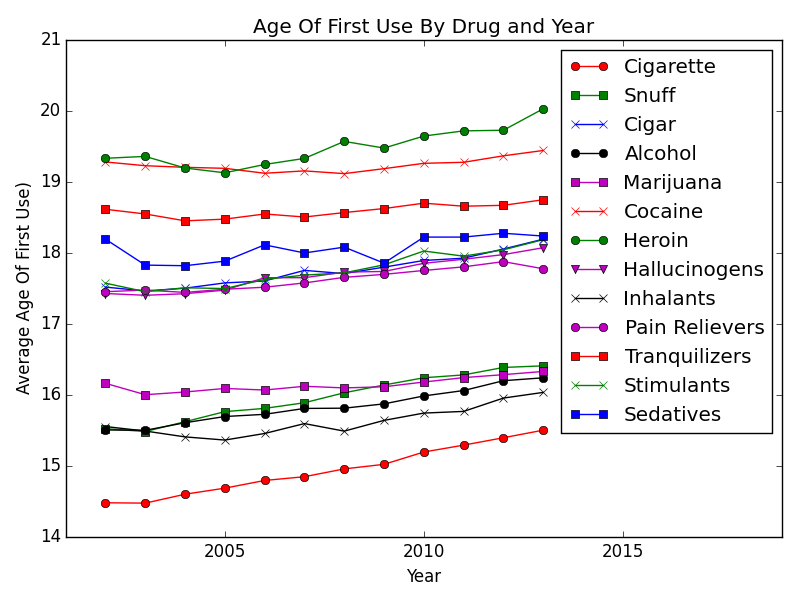
\includegraphics[width=\textwidth]{avgAFU_02-13}

\noindent The above plot displays the mean age of first use for a number of popular drugs over time. The most important feature with respect to targeted education is the fact that the mean age of first use for all drugs is between 15 and 20, and the mean age of first use for the most popular drugs (nicotine products, alcohol, and marijuana) is between 15 and 16. This indicates that most drug education efforts should be targeted at teens, and specifically at 14,15, and 16 year-olds (in order to maximize drug use prevention).\\

\noindent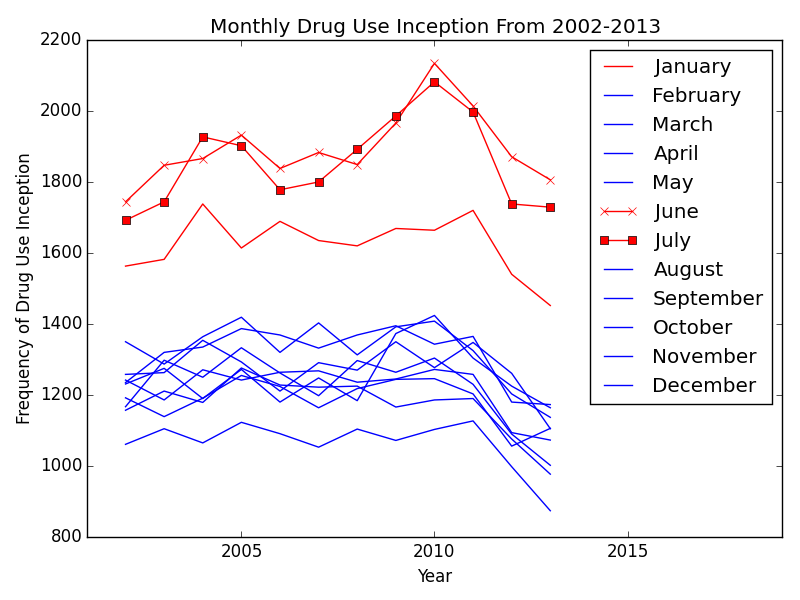
\includegraphics[width=\textwidth]{mfu_02-13}

\noindent The above plot displays the frequency of drug use inception of each month from January 2002 through December of 2013. January, June, and July feature significantly higher frequencies than the other months, indicating that drug education and anti-drug advertising should be dispersed in December, May, and June for increased drug use prevention.

\subsection*{How Much Do These Drugs Affect The Rest Of Us?}
Moving back towards the SII, we now inspect the usage of substance abuse treatment services by various drug user populations.\\

\noindent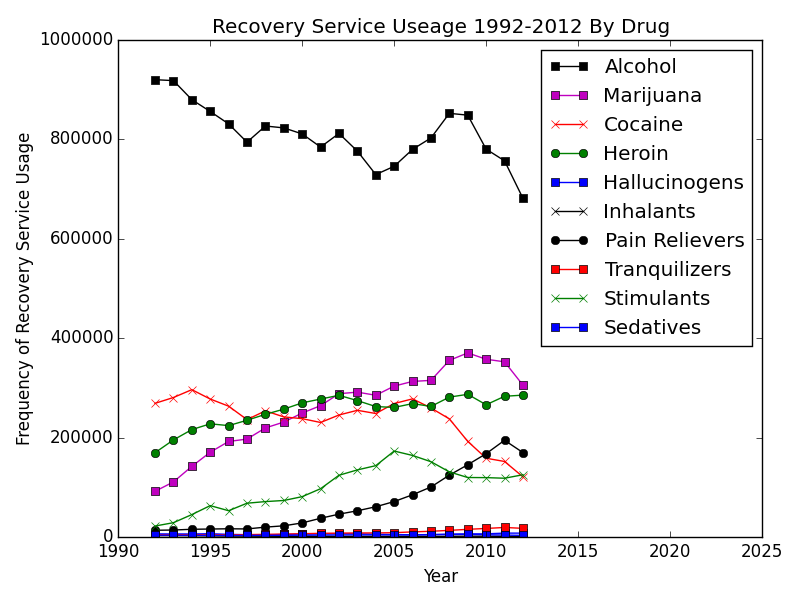
\includegraphics[width=\textwidth]{TEDS-A_92-12}

\noindent Back in the 90's, alcohol, cocaine, and heroin users utilized the most substance abuse treatment services. In more recent times though this has shifted to alcohol, marijuana, heroin, and pain relievers. Alcohol and cocaine users have been using less abuse services, most likely due to decreased population size. Users of pain relievers have been utilizing an increasing amount of these services, with the growth showing a super linear trend until a small decrease appeared in 2012.\\

\noindent The final piece of the puzzle required for the SII calculation is the usage of emergency services by various drug user populations.\\

\noindent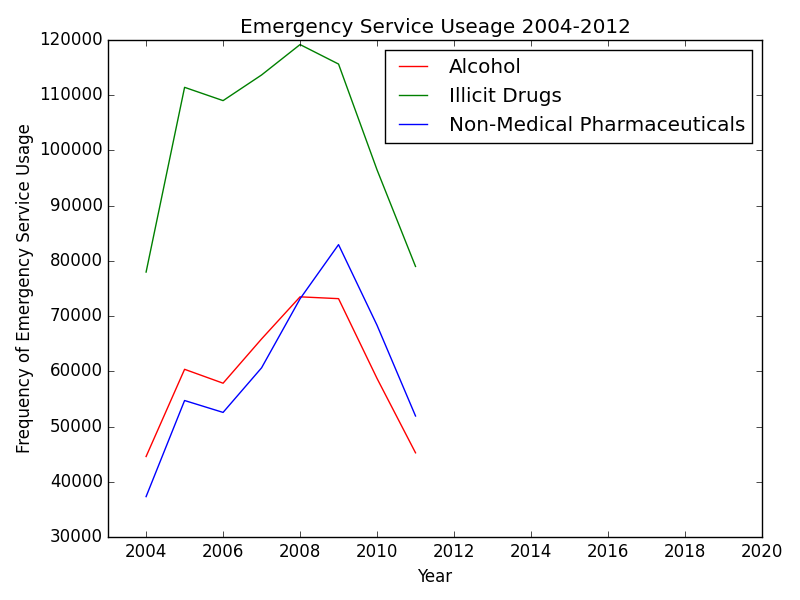
\includegraphics[width=\textwidth]{DAWN_04-11}

\noindent Unfortunately, data in this area was limited in both breadth and depth. Thus the categories of drugs was reduced along with the number of years that data was available for. Despite the general lack of data, there are still important pieces of knowledge which can be gleaned from this plot. First, it is important to not that illicit drugs account for almost double the emergency service use as alcohol or pharmaceuticals. Second, there is a large spike  in 2009 and 2010 which falls of rapidly in 2011. This spike is mirrored in a number of the plots displayed thus far and investigation into its source could bring valuable insights into more powerful methods of altering drug usage in the U.S.\\

\noindent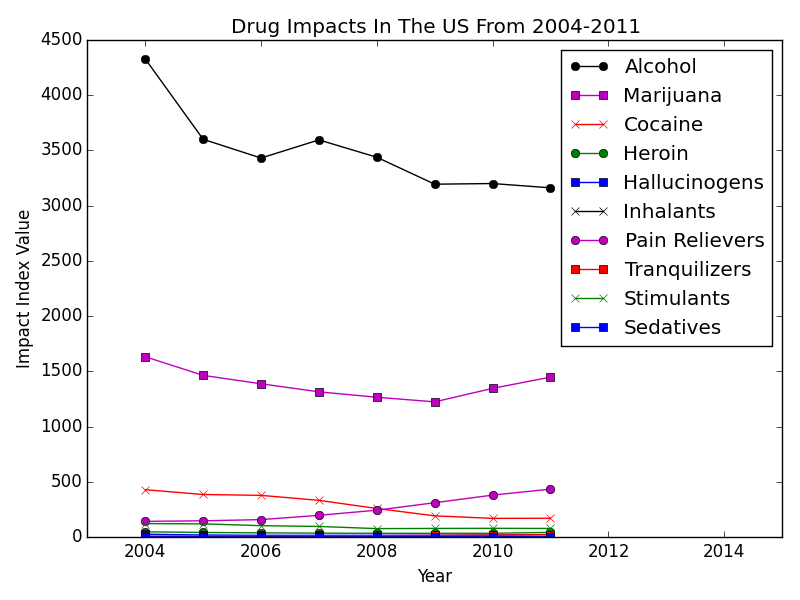
\includegraphics[width=\textwidth]{impactIndex}

\noindent The final plot displays the SII calculation for 2004 through 2011, which were the years that emergency services data was available for. Note that nicotine products were omitted from this plot as the number of nicotine related emergency service uses were extremely small compared to the drugs presented. Alcohol and marijuana clearly dominate the plot, with cocaine and pain relievers a short distance behind. 

\section*{Discussion}
\subsection*{Important Results}
\noindent The plots presented serve to reinforce many of the findings of my mid-term paper, showing that the results found hold over many years with only slight variation. Other important findings include many gradual transitions in drug behaviors including the general decline of many drug user populations, the ascent of the average age of first use for all drugs presented, an increase in drug abuse treatment services by marijuana, heroin, and pain reliever users, and the creation of a crude impact index (the SII) which has room for growth and improvement. Another interesting trend is the moderate spike in many drug activities in 2010 and subsequent fall in the following years.

\subsection*{Future Work}
\noindent A number of interesting behaviors were discovered, however there remain many more left to be uncovered. Some notable avenues for future work are the refinement of the SII in order to increase accuracy and the number of drugs covered, investigation and comparison of drug use behavior in other countries, refinement of emergency service usage data, and investigation into what factors increase the risk for drug use.


\pagebreak


\begin{thebibliography}{1}
	\bibitem{Anti-Drug Money} "Anti-Drug Campaign Research - Futures of Palm Beach." Futures of Palm Beach. Web. 13 Dec. 2015. \textcolor{blue}{http://www.futuresofpalmbeach.com/anti-drug-campaign-research/\#\textunderscore ftn10}
	
	\bibitem{NSDUH13} United States Department of Health and Human Services. Substance Abuse and Mental Health Services Administration. Center for Behavioral Health Statistics and Quality. National Survey on Drug Use and Health, 2013. ICPSR35509-v3. Ann Arbor, MI: Inter-university Consortium for Political and Social Research [distributor], 2015-11-23. \textcolor{blue}{http://doi.org/10.3886/ICPSR35509.v3}
	
	\bibitem{NSDUH12} United States Department of Health and Human Services. Substance Abuse and Mental Health Services Administration. Center for Behavioral Health Statistics and Quality. National Survey on Drug Use and Health, 2012. ICPSR34933-v2. Ann Arbor, MI: Inter-university Consortium for Political and Social Research [distributor], 2014-10-06. \textcolor{blue}{http://doi.org/10.3886/ICPSR34933.v2}
	
	\bibitem{NSDUH11} United States Department of Health and Human Services. Substance Abuse and Mental Health Services Administration. Center for Behavioral Health Statistics and Quality. National Survey on Drug Use and Health, 2011. ICPSR34481-v4. Ann Arbor, MI: Inter-university Consortium for Political and Social Research [distributor], 2015-11-23. \textcolor{blue}{http://doi.org/10.3886/ICPSR34481.v4}
	
	\bibitem{NSDUH10} United States Department of Health and Human Services. Substance Abuse and Mental Health Services Administration. Center for Behavioral Health Statistics and Quality. National Survey on Drug Use and Health, 2010. ICPSR32722-v6. Ann Arbor, MI: Inter-university Consortium for Political and Social Research [distributor], 2015-11-23. \textcolor{blue}{http://doi.org/10.3886/ICPSR32722.v6}
	
	\bibitem{NSDUH09} United States Department of Health and Human Services. Substance Abuse and Mental Health Services Administration. Office of Applied Studies. National Survey on Drug Use and Health, 2009. ICPSR29621-v6. Ann Arbor, MI: Inter-university Consortium for Political and Social Research [distributor], 2015-11-23. \textcolor{blue}{http://doi.org/10.3886/ICPSR29621.v6}
	
	\bibitem{NSDUH08} United States Department of Health and Human Services. Substance Abuse and Mental Health Services Administration. Office of Applied Studies. National Survey on Drug Use and Health, 2008. ICPSR26701-v6. Ann Arbor, MI: Inter-university Consortium for Political and Social Research [distributor], 2015-11-23. \textcolor{blue}{http://doi.org/10.3886/ICPSR26701.v6}
	
	\bibitem{NSDUH07} United States Department of Health and Human Services. Substance Abuse and Mental Health Services Administration. Office of Applied Studies. National Survey on Drug Use and Health, 2007. ICPSR23782-v5. Ann Arbor, MI: Inter-university Consortium for Political and Social Research [distributor], 2015-11-23. \textcolor{blue}{http://doi.org/10.3886/ICPSR23782.v5}
	
	\bibitem{NSDUH06} United States Department of Health and Human Services. Substance Abuse and Mental Health Services Administration. Office of Applied Studies. National Survey on Drug Use and Health, 2006. ICPSR21240-v6. Ann Arbor, MI: Inter-university Consortium for Political and Social Research [distributor], 2013-06-21. \textcolor{blue}{http://doi.org/10.3886/ICPSR21240.v6}
	
	\bibitem{NSDUH05} United States Department of Health and Human Services. Substance Abuse and Mental Health Services Administration. Office of Applied Studies. National Survey on Drug Use and Health, 2005. ICPSR04596-v5. Ann Arbor, MI: Inter-university Consortium for Political and Social Research [distributor], 2015-11-23. \textcolor{blue}{http://doi.org/10.3886/ICPSR04596.v5}
	
	\bibitem{NSDUH04} United States Department of Health and Human Services. Substance Abuse and Mental Health Services Administration. Office of Applied Studies. National Survey on Drug Use and Health, 2004. ICPSR04373-v4. Ann Arbor, MI: Inter-university Consortium for Political and Social Research [distributor], 2015-11-23. \textcolor{blue}{http://doi.org/10.3886/ICPSR04373.v4}
	
	\bibitem{NSDUH03} United States Department of Health and Human Services. Substance Abuse and Mental Health Services Administration. Office of Applied Studies. National Survey on Drug Use and Health, 2003. ICPSR04138-v5. Ann Arbor, MI: Inter-university Consortium for Political and Social Research [distributor], 2015-11-23. \textcolor{blue}{http://doi.org/10.3886/ICPSR04138.v5}
	
	\bibitem{NSDUH02} United States Department of Health and Human Services. Substance Abuse and Mental Health Services Administration. Office of Applied Studies. National Survey on Drug Use and Health, 2002. ICPSR03903-v6. Ann Arbor, MI: Inter-university Consortium for Political and Social Research [distributor], 2015-11-23. \textcolor{blue}{http://doi.org/10.3886/ICPSR03903.v6}
	
	\bibitem{DAWN11} United States Department of Health and Human Services. Substance Abuse and Mental Health Services Administration. Center for Behavioral Health Statistics and Quality. Drug Abuse Warning Network (DAWN), 2011. ICPSR34565-v3. Ann Arbor, MI: Inter-university Consortium for Political and Social Research [distributor], 2015-11-23. \textcolor{blue}{http://doi.org/10.3886/ICPSR34565.v3}
	
	\bibitem{DAWN10} United States Department of Health and Human Services. Substance Abuse and Mental Health Services Administration. Center for Behavioral Health Statistics and Quality. Drug Abuse Warning Network (DAWN), 2010. ICPSR34083-v3. Ann Arbor, MI: Inter-university Consortium for Political and Social Research [distributor], 2015-11-23. \textcolor{blue}{http://doi.org/10.3886/ICPSR34083.v3}
	
	\bibitem{DAWN09} United States Department of Health and Human Services. Substance Abuse and Mental Health Services Administration. Center for Behavioral Health Statistics and Quality. Drug Abuse Warning Network (DAWN), 2009. ICPSR31921-v4. Ann Arbor, MI: Inter-university Consortium for Political and Social Research [distributor], 2015-11-23. \textcolor{blue}{http://doi.org/10.3886/ICPSR31921.v4}
	
	\bibitem{DAWN08} United States Department of Health and Human Services. Substance Abuse and Mental Health Services Administration. Center for Behavioral Health Statistics and Quality. Drug Abuse Warning Network (DAWN), 2008. ICPSR31264-v6. Ann Arbor, MI: Inter-university Consortium for Political and Social Research [distributor], 2015-11-23. \textcolor{blue}{http://doi.org/10.3886/ICPSR31264.v6}
	
	\bibitem{DAWN07} United States Department of Health and Human Services. Substance Abuse and Mental Health Services Administration. Office of Applied Studies. Drug Abuse Warning Network (DAWN), 2007. ICPSR32861-v4. Ann Arbor, MI: Inter-university Consortium for Political and Social Research [distributor], 2015-11-23. \textcolor{blue}{http://doi.org/10.3886/ICPSR32861.v4}
	
	\bibitem{DAWN06} United States Department of Health and Human Services. Substance Abuse and Mental Health Services Administration. Office of Applied Studies. Drug Abuse Warning Network (DAWN), 2006. ICPSR33221-v3. Ann Arbor, MI: Inter-university Consortium for Political and Social Research [distributor], 2015-11-23. \textcolor{blue}{http://doi.org/10.3886/ICPSR33221.v3}
	
	\bibitem{DAWN05} United States Department of Health and Human Services. Substance Abuse and Mental Health Services Administration. Office of Applied Studies. Drug Abuse Warning Network (DAWN), 2005. ICPSR33042-v3. Ann Arbor, MI: Inter-university Consortium for Political and Social Research [distributor], 2015-11-23. \textcolor{blue}{http://doi.org/10.3886/ICPSR33042.v3}
	
	\bibitem{DAWN04} United States Department of Health and Human Services. Substance Abuse and Mental Health Services Administration. Office of Applied Studies. Drug Abuse Warning Network (DAWN), 2004. ICPSR33041-v3. Ann Arbor, MI: Inter-university Consortium for Political and Social Research [distributor], 2015-11-23. \textcolor{blue}{http://doi.org/10.3886/ICPSR33041.v3}
	
	
	\bibitem{TEDS-A} United States Department of Health and Human Services. Substance Abuse and Mental Health Services Administration. Center for Behavioral Health Statistics and Quality. Treatment Episode Data Set -- Admissions (TEDS-A) -- Concatenated, 1992 to 2012. ICPSR25221-v10. Ann Arbor, MI: Inter-university Consortium for Political and Social Research [distributor], 2015-11-23. \textcolor{blue}{http://doi.org/10.3886/ICPSR25221.v10}
	
\end{thebibliography}

\end{document}
